\achapter{32}{Bases for Vector Spaces} \label{sec:bases}

\vspace*{-17 pt}
\framebox{
\parbox{\dimexpr\linewidth-3\fboxsep-3\fboxrule}
{\begin{fqs}
\item What does it mean for a set $\{\vv_1, \vv_2, \ldots, \vv_k\}$ of vectors in a vector space $V$ to be linearly independent? 
\item What is another equivalent characterization of a linearly independent set? 
\item What does is mean for a set $\{\vv_1, \vv_2, \ldots, \vv_k\}$ of vectors in a vector space $V$ to be linearly dependent? 
\item Describe another characterization of a linearly dependent set.
\item What is a basis for a vector space $V$? 
\item What makes a basis for a vector space useful?
\item How can we find a basis for a vector space $V$? 
\end{fqs}}}% \hspace*{3 pt}}

\vspace*{13 pt}

\csection{Application: Image Compression}

\begin{quote} If you painted a picture with a sky, clouds, trees, and flowers, you would use a different size brush depending on the size of the features. Wavelets are like those brushes.
\end{quote}
\vspace{-0.20in} 
\hspace{0.35in} $-$ Ingrid Daubechies

The advent of the digital age has presented many new opportunities for the collection, analysis,  and dissemination of information. Along with these opportunities come new difficulties as well. All of this digital information must be stored in some way and be retrievable in an efficient manner. One collection of tools that is used to deal with these problems is wavelets. For example, the FBI fingerprint files contain millions of cards, each of which contains 10 rolled fingerprint impressions. Each card produces about 10 megabytes of data. To store all of these cards would require an enormous amount of space, and transmitting one full card over existing data lines is slow and inefficient. Without some sort of image compression, a sortable and searchable electronic fingerprint database would be next to impossible. To deal with this problem, the FBI adopted standards for fingerprint digitization using a wavelet compression standard. 

 Another problem with electronics is noise. Noise can be a big problem when collecting and transmitting data. Wavelet decomposition filters data by averaging and detailing. The detailing coefficients indicate where the details are in the original data set. If some details are very small in relation to others, eliminating them may not substantially alter the original data set. Similar ideas may be used to restore damaged audio,\footnote{see \url{https://ccrma.stanford.edu/groups/edison/brahms/brahms.html} for a discussion of the denoising of a Brahms recording} video, photographs, and medical information.\footnote{A review of wavelets in biomedical applications.  M. Unser, A. Aldroubi. \emph{Proceedings of the IEEE}, Volume: 84, Issue: 4 , Apr 1996}

We will consider wavelets as a tool for image compression. The basic idea behind using wavelets to compress images is that we start with a digital image, made up of pixels. Each pixel can be assigned a number or a vector (depending on the makeup of the image). The image can then be represented as a matrix (or a set of matrices) $M$, where each entry in $M$ represents a pixel in the image. As a simple example, consider the $16 \times 16$ image of a flower as shown at left in Figure \ref{F:Flower_1}. (We will work with small images like this to make the calculations more manageable, but the ideas work for any size image. We could also extend our methods to consider color images, but for the sake of simplicity we focus on grayscale.) 
\begin{figure}[h]
\begin{center}
\resizebox{!}{2.25in}{
\includegraphics{flower}} \hspace{0.1in} \resizebox{!}{2.25in}{\includegraphics{flower_2}}
\end{center}
\caption{Left: A 16 by 16 pixel image. Right: The image compressed.}
\label{F:Flower_1}
\end{figure}
This flower image is a gray-scale image, so each pixel has a numeric representation between 0 and 255, where 0 is black,  255 is white, and numbers between 0 and 255 represent shades of gray. The matrix for this flower image is 
\begin{equation} \label{eq:flower_image_matrix} 
 \left[\arraycolsep=2.5pt {\scriptsize \begin{array}{cccccccccccccccc} 240&240&240&240&130&130&240&
130&130&240&240&240&240&240&240&240\\240&240&240&130
&175&175&130&175&175&130&240&240&240&240&240&240\\
240&240&130&130&175&175&130&175&175&130&130&240&240&240&240&240
\\240&130&175&175&130&175&175&175&130&175&175&130&
240&240&240&240\\240&240&130&175&175&130&175&130&175
&175&130&240&240&240&240&240\\255&240&240&130&130&
175&175&175&130&130&240&240&225&240&240&240\\240&240
&130&175&175&130&130&130&175&175&130&240&225&255&240&240
\\240&240&130&175&130&240&130&240&130&175&130&240&
255&255&255&240\\240&240&240&130&240&240&75&240&240&
130&240&255&255&255&255&255\\240&240&240&240&240&240
&75&240&240&240&240&240&240&240&240&240\\240&240&240
&75&75&240&75&240&75&75&240&240&240&240&240&240\\50&
240&240&240&75&240&75&240&75&240&240&240&240&50&240&240
\\240&75&240&240&240&75&75&75&240&240&50&240&50&240&
240&50\\240&240&75&240&240&240&75&240&240&50&240&50&
240&240&50&240\\75&75&75&75&75&75&75&75&75&75&75&75&
75&75&75&75\\75&75&75&75&75&75&75&75&75&75&75&75&75&
75&75&75\end {array} }\right].
\end{equation} 

Now we can apply wavelets to the image and compress it. Essentially, wavelets act by averaging and differencing. The averaging creates smaller versions of the image and the differencing keeps track of how far the smaller version is from a previous copy. The differencing often produces many small (close to 0) entries, and so replacing these entries with 0 doesn't have much effect on the image (this is called \emph{thresholding}). By introducing long strings of zeros into our data, we are able to store a (compressed) copy of the image in a smaller amount of space. For example, using a threshold value of 10 produces the flower image shown at right in Figure \ref{F:Flower_1}. 

The averaging and differencing is done with special vectors (wavelets) that form a basis for a suitable function space. More details of this process can be found at the end of this section. 


\csection{Introduction}

In $\R^n$ we defined a basis for a subspace $W$ of $\R^n$ to be a minimal spanning set for $W$, or a linearly independent spanning set (see Definition \ref{def:1_f_basis}). So to consider the idea of a basis in a vector space, we will need the notion of linear independence in that context. 

Since we can add vectors and multiply vectors by scalars in any vector space, and because we have a zero vector in any vector space, we can define linear independence of a finite set of vectors in any vector space as follows (compare to Definition \ref{def:linear_independence_Rn}). 


\begin{definition} \label{def:vs_linear_independence} A set $\{\vv_1, \vv_2, \ldots, \vv_k\}$ of vectors in a vector space $V$ is \textbf{linearly independent}\index{linearly independent vectors in a vector space} if the vector equation
\[x_1 \vv_1 + x_2 \vv_2 + \cdots + x_k \vv_k = \vzero\]
for scalars $x_1, x_2, \ldots, x_k$ has only the trivial solution
\[x_1 = x_2 = x_3 = \cdots = x_k = 0.\]
If a set of vectors is not linearly independent, then the set is \textbf{linearly dependent}\index{linear dependent vectors in a vector space}.
\end{definition}

Alternatively, we say that the vectors $\vv_1, \vv_2, \ldots, \vv_k$ are linearly independent (or dependent) if the set $\{\vv_1, \vv_2, \ldots, \vv_k\}$ is linearly independent (or dependent).



\begin{pa} \label{pa:5_b}  ~
\be
\item We can use the tools we developed to determine if a set of vectors in $\R^n$ is linearly independent to answer the same questions for sets of vectors in other vector spaces. For example, consider the question of whether the set $\{1+t, 1-t\}$ in $\pol_1$ is linearly independent or dependent. To answer this question we need to determine if there is a non-trivial solution to the equation
\begin{equation} \label{eq:PA_5_b_1}
x_1 (1+t) + x_2(1-t) = 0.
\end{equation}
Note that equation (\ref{eq:PA_5_b_1}) can also be written in the form
\[(x_1+x_2) + (x_1-x_2)t = 0.\]
	\ba
	\item Recall that two polynomials are equal if all coefficients of like powers are the same. By equating coefficients of like power terms, rewrite equation (\ref{eq:PA_5_b_1}) as an equivalent system of two equations in the two unknowns $x_1$ and $x_2$, and solve for $x_1, x_2$. 

	
	
	\item What does your answer to the previous part tell you about the linear independence or dependence of the set $\{1+t, 1-t\}$ in $\pol_1$?

\item Recall that in $\R^n$, a set of two vectors is linearly dependent if and only if one of the vectors in the set is a scalar multiple of the other and linearly independent if neither vector is a scalar multiple of the other. Verify your answer to part (c) from a similar perspective in $\pol_1$.

	\ea

\item We can use the same type of method as in problem (1) to address the question of whether the set 
\[\left\{ \left[ \begin{array}{cc} 1&3 \\ 1&2 \end{array} \right], \left[ \begin{array}{cr} 1&-9 \\ 1&8 \end{array} \right], \left[ \begin{array}{cr} 1&-1 \\ 1&4 \end{array} \right] \right\}\]
is linearly independent or dependent in $\M_{2 \times 2}$. To answer this question we need to determine if there is a non-trivial solution to the equation
\begin{equation} \label{eq:PA_5_b_2}
x_1\left[ \begin{array}{cc} 1&3 \\ 1&2 \end{array} \right] + x_2\left[ \begin{array}{cr} 1&-9 \\ 1&8 \end{array} \right] + x_3 \left[ \begin{array}{cr} 1&-1 \\ 1&4 \end{array} \right] = \vzero
\end{equation}
for some scalars $x_1$, $x_2$, and $x_3$.  Note that the linear combination on the left side of equation (\ref{eq:PA_5_b_2}) has entries
\[\left[ \begin{array}{cc} x_1+x_2+x_3&3x_1-9x_2-x_3 \\ x_1+x_2+x_3&2x_1+8x_2+4x_3 \end{array} \right].\]
	\ba
	\item Recall that two matrices are equal if all corresponding entries are the same. Equate corresponding entries of the matrices in equation (\ref{eq:PA_5_b_2}) to rewrite the equation as an equivalent system of four equations in the three unknowns $x_1$, $x_2$, and $x_3$. 



	\item Use appropriate matrix tools and techniques to find all solutions to the system from part (a).
	
	
	\item What does the set of solutions to the system from part (a) tell you about the linear independence or dependence of the set 
\[\left\{ \left[ \begin{array}{cc} 1&3 \\ 1&2 \end{array} \right], \left[ \begin{array}{cr} 1&-9 \\ 1&8 \end{array} \right], \left[ \begin{array}{cr} 1&-1 \\ 1&4 \end{array} \right] \right\}?\]
	


\item Recall that in $\R^n$, a set of vectors is linearly dependent if and only if one of the vectors in the set is a linear combination of the others and linearly independent if no vector in the set is a linear combination of the others. Verify your answer to part (c) from a similar perspective in $\M_{2 \times 2}$.
 	
	\ea
	
	
\item We will define a basis for a vector space to be a linearly independent spanning set. Which, if any, of the sets in parts (1) and (2) is a basis for its vector space? Explain. 

\ee

\end{pa}

\csection{Linear Independence}

The concept of linear independence, which we formally defined in Preview Activity \ref{pa:5_b}, provides us with a process to determine if there is redundancy in a spanning set to obtain an efficient spanning set. 


The definition tells us that a set $\{\vv_1, \vv_2, \ldots, \vv_k\}$ of vectors in a vector space $V$ is linearly dependent if there are scalars $x_1$, $x_2$, $\ldots$, $x_n$, not all of which are 0 so that
\[x_1 \vv_1 + x_2 \vv_2 + \cdots + x_k \vv_k = \vzero.\]

As examples, we saw in Preview Activity \ref{pa:5_b} that the set $\{1+t, 1-t\}$ is linearly independent in $\pol_1$. The set $\{1+t, -1+2t+t^2, 1-8t-3t^2\}$, on the other hand, is linearly dependent in $\pol_2$ since $2(1+t) + 3(-1+2t+t^2) + (1-8t-3t^2) = 0$.  

In addition to the definition, there are other ways to characterize linearly independent and dependent sets in vector spaces as the next theorems illustrate. These characterizations are the same as those we saw in $\R^n$, and the proofs are essentially the same as well. The proof of Theorem \ref{thm:5_b_1} is similar to that of Theorem \ref{thm:Dependence} and is left for the exercises. 

\begin{theorem} \label{thm:5_b_1} A set $\{\vv_1, \vv_2, \ldots, \vv_k\}$ of vectors in a vector space $V$ is linearly dependent if and only if at least one of the vectors in the set can be written as a linear combination of the remaining vectors in the set.
\end{theorem}

Theorem \ref{thm:5_b_1} is equivalent to the following theorem that provides the corresponding result for linearly independent sets.  

\begin{theorem} \label{thm:5_b_2} A set $\{\vv_1, \vv_2, \ldots, \vv_k\}$ of vectors in a vector space $V$ is linearly independent if and only if no vector in the set can be written as a linear combination of the remaining vectors in the set.
\end{theorem}


One consequence of Theorems \ref{thm:5_b_1} and \ref{thm:5_b_2} is that if a spanning set is linearly dependent, then one of the vectors in the set can be written as a linear combination of the others. In other words, at least one of the vectors is redundant. In that case, we can find a smaller spanning set as the next theorem states. The proof of this theorem is similar to that of Theorem \ref{thm:minimal_spanning_set} and is left for the exercises. 

\begin{theorem} \label{thm:5_b_3} Let $\{\vv_1, \vv_2, \ldots, \vv_k\}$ be a set of vectors in a vector space $V$. If for some $i$ between 1 and $k$, $\vv_i$ is in $\Span \{\vv_1, \vv_2, \ldots, \vv_{i-1}, \vv_{i+1}, \ldots, \vv_k\}$, then
\[\Span\{\vv_1, \vv_2, \ldots, \vv_k\} = \Span\{\vv_1, \vv_2, \ldots, \vv_{i-1}, \vv_{i+1}, \ldots, \vv_k\}.\]
\end{theorem}


\csection{Bases}

A basis for a vector space is a spanning set that is as small as it can be. We already saw how to define bases formally in $\R^n$. We will now formally define a basis for a vector space and understand why with this definition a basis is a minimal spanning set. Bases are important because any vector in a vector space can be uniquely represented as a linear combination of basis vectors. We will see in later sections that this representation will allow us to identify any vector space with a basis of $n$ vectors with $\R^n$. 


To obtain the formal definition of a basis, which is a minimal spanning set, we consider what additional property makes a spanning set a \emph{minimal} spanning set. As a consequence of Theorem \ref{thm:5_b_3}, if $S$ is a spanning set that is linearly dependent, then we can find a proper subset of $S$ that has the same span. Thus, the set $S$ cannot be a minimal spanning set. However, if $S$ is linearly independent, then no vector in $S$ is a linear combination of the others and we need all of the vectors in $S$ to form the span. This leads us to the following formal characterization of a minimal spanning set, called a \emph{basis}.


\begin{definition} A \textbf{basis}\index{basis for a vector space}\index{vector space!basis} for a vector space $V$ is a subset $S$ of $V$ if
\begin{enumerate}
\item $\Span \ S = V$ and
\item $S$ is a linearly independent set.
\end{enumerate}
\end{definition}



In other words, a basis for a vector space $V$ is a linearly independent spanning set for $V$. To put it another way, a basis for a vector space is a minimal spanning set for the vector space. Similar reasoning will show that a basis is also a maximal linearly independent set.


The key ideas to take from the previous theorems are:
\begin{itemize}
\item A basis for a vector space $V$ is a minimal spanning set for $V$.
\item A basis for $V$ is a subset $S$ of $V$ so that
    \begin{enumerate}
    \item $S$ spans $V$ and
    \item $S$ is linearly independent.
    \end{enumerate}
\item No vector in a basis can be written as a linear combination of the other vectors in the basis.
\item If a subset $S$ of a vector space $V$ has the property that one of the vectors in $S$ is a linear combination of the other vectors in $S$, then $S$ is not a basis for $V$.
\end{itemize}



As an example of a basis of a vector space, we saw in Preview Activity \ref{pa:5_b} that the set $S = \{1-t, 1+t\}$ is both linearly independent and spans $\pol_1$, and so $S$ is a basis for $\pol_1$. 



\begin{activity} \label{act:5_b_1} ~
	\ba
	\item Is $S = \{1+t, t, 1-t\}$ a basis for $\pol_1$? Explain.
%	\item Is $S = \{1+3t+t^2, 2+4t+t^2, 1+t+t^2, 3+5t+2t^2\}$ a basis for $\pol_2$? Explain.



	\item Explain why the set $S = \{1, t, t^2, \ldots, t^n\}$ is a basis for $\pol_n$. This basis is called the \emph{standard basis}\index{standard basis!for $\pol_n$} for $\pol_n$.



	\item Show that the set 
	\[\left\{ \left[ \begin{array}{cc} 1&0 \\ 1&1 \end{array} \right], \left[ \begin{array}{cc} 0&1 \\ 1&1 \end{array} \right], \left[ \begin{array}{cc} 1&1 \\ 1&0 \end{array} \right], \left[ \begin{array}{cc} 1&1 \\ 0&1 \end{array} \right] \right\}\]
	is a basis for $\M_{2 \times 2}$. 

	\ea
\end{activity}



It should be noted that not every vector space has a finite basis. For example, the space $\pol$ of all polynomials with real coefficients (of any degree) is a vector space, but no finite set of vectors will span $\pol$. In fact, the infinite set $\{1, t, t^2, \ldots\}$ is both linearly independent and spans $\pol$, so $\pol$ has an infinite basis. 

\csection{Finding a Basis for a Vector Space}

We already know how to find bases for certain vector spaces, namely $\Nul A$ and $\Col A$, where $A$ is any matrix. Finding a basis for a different kind of vector space will require other methods. Since a basis for a vector space is a minimal spanning set, to find a basis for a given vector space we might begin from scratch, starting with a given vector in the space and adding one vector at a time until we have a spanning set. 

\begin{activity} \label{act:5_b_2} Let $W = \{a + bt + ct^3 \mid a, b, c \text{ are scalars}\}$. We will find a basis of $W$ that contains the polynomial $3+t-t^3$. 
	\ba	
	\item Let $\CS_1 = \{3+t-t^3\}$. Find a polynomial $p(t)$ in $W$ that is not in $\Span \ \CS_1$. Explain why this means that the set $\CS_1$ does not span $W$.
	
	\item  Let $\CS_2 = \{3+t-t^3, p(t)\}$. Find a polynomial $q(t)$ that is not in $\Span \ \CS_2$. What does this mean about $\CS_2$ being a possible spanning set of $W$? 
		
	\item  Let $\CS_3 = \{3+t-t^3, p(t), q(t)\}$. Explain why the set $\CS_3$ is a basis for $W$. 

	\ea

\end{activity}

Alternatively, we might construct a basis from a known spanning set.

\begin{activity}  \label{act:5_b_2_b}  Let $W = \left\{\left[ \begin{array}{cc} v+z&w+z \\ x&y \end{array} \right] \left. \right| v, w, x, y, z \text{ are scalars}\right\}$. Assume that $W$ is a subspace of $\M_{2 \times 2}$. 
	\ba
	\item Find a set $S$ of five $2 \times 2$ matrices that spans $W$ (since $W$ is a span of a set of vectors in $\M_{2 \times 2}$, $W$ is a subspace of $\M_{2 \times 2}$). Without doing any computation, can this set $S$ be a basis for $W$? Why or why not?
	
	
	
	\item Find a subset $\CB$ of $S$ that is a basis for $W$.

	\ea
	
\end{activity}



Activities \ref{act:5_b_2} and \ref{act:5_b_2_b} give us two ways of finding a basis for a subspace $W$ of a vector space $V$, assuming $W$ has a basis with finitely many vectors. One way (illustrated in Activity \ref{act:5_b_2})  is to start by choosing any non-zero vector $\vw_1$ in $W$. Let $\CS_1 = \{\vw_1\}$. If $\CS_1$ spans $W$, then $\CS_1$ is a basis for $W$. If not, there is a vector $\vw_2$ in $W$ that is not in $\Span \ \CS_1$. Then $\CS_2 = \{\vw_1, \vw_2\}$ is a linearly independent set. If $\Span \ \CS_2 = W$, then $\CS_2$ is a basis for $W$ and we are done. If not, repeat the process. We will show later that this process must stop as long as we know that $W$ has a basis with finitely many vectors. 

Another way (illustrated in Activity \ref{act:5_b_2_b})  to find a basis for $W$ is to start with a spanning set $\CS_1$ of $W$. If $\CS_1$ is linearly independent, then $\CS_1$ is a basis for $W$. If $\CS_1$ is linearly dependent, then one vector in $\CS_1$ is a linear combination of the others and we can remove that vector to obtain a new set $\CS_2$ that also spans $W$. If $\CS_2$ is linearly independent, then $\CS_2$ is a basis for $W$. If not, we repeat the process as many times as needed until we arrive until at a subset $\CS_k$ of $\CS_1$ that is linearly independent and spans $W$. We summarize these results in the following theorem.  

\begin{theorem} Let $W$ be a subspace of a finite-dimensional vector space $V$. Then
\begin{enumerate}
\item any linearly independent subset of $W$ can be extended to a basis of $W$,
\item any subset of $W$ that spans $W$ can be reduced to a basis of $W$.
\end{enumerate}
\end{theorem}


We conclude this section with the result mentioned in the introduction -- that every vector in a vector space with basis $\B$ can be written in one and only one way as a linear combination of basis vectors. The proof is similar to that of Theorem \ref{thm:1_f_unique_representation} and is left to the exercises. 



\begin{theorem} \label{thm:5_b_4} Let $\vv_1$, $\vv_2$, $\ldots$, $\vv_n$ be vectors in a vector space $V$ that make up a basis $\B$ for $V$. If $\vu$ is a vector in $V$, then $\vu$ can be written in one and only one way as a linear combination of vectors $\vv_1$, $\vv_2$, $\ldots$, $\vv_n$ in $\B$. 
\end{theorem}

\csection{Examples}

\ExampleIntro 

\begin{example} Let $S = \{1, 1+t, 2-t^2, 1+t+t^2, t-t^2\}$. 
	\ba
	\item Does $S$ span $\pol_2$? Explain.
	
	\item Explain why $S$ is not a basis for $\pol_2$.
	
	\item Find a subset of $S$ that is a basis for $\pol_2$. Explain your reasoning.
	
	\ea

\ExampleSolution
	\ba
	\item Let $p(t) = a_0+a_1t+a_2t^2$ be an arbitrary vector in $\pol_2$. If $p(t)$ is in $\Span \ S$, then there are weights $c_1$, $c_2$, $c_3$, $c_4$, and $c_5$ such that 
	\[a_0+a_1t+a_2t^2 = c_1(1) + c_2(1+t) + c_3(2-t^2) + c_4(1+t+t^2) + c_5(t-t^2).\]
	Equating coefficients of like powers gives us the system
	\begin{alignat*}{6}
{}c_1 	&{}+{} 	&{}c_2 	&{}+{}	&{2}c_3	&{}+{}	&{}c_4	&{}{}	&{} 		&= a_0&{} \\
{} 		&{}{} 		&{}c_2 	&{}{}		&{}		&{}+{}	&{}c_4	&{}+{}	&{}c_5 		&= a_1&{} \\
{} 		&{}{} 		&{} 		&{}{}		&{-}c_3	&{}+{}	&{}c_4	&{}-{}	&{}c_5 		&= a_2&{.} 
\end{alignat*}
The reduced row echelon form of the coefficient matrix $A$ is 
\[\left[ \begin{array}{cccrr} 1&0&0&2&-3 \\ 0&1&0&1&1 \\ 0&0&1&-1&1 \end{array} \right].\]
Since there is a pivot in every row of $A$, the system $A \vx = \vb$ is always consistent. We conclude that $S$ does span $\pol_2$. 
	
	
	\item The fact that the coefficient matrix $A$ of our system has non-pivot columns means that each vector in $\pol_2$ can be written in more than one way as a linear combination of vectors in $S$. This means that $S$ is not linearly independent and so cannot be a basis for $\pol_2$.  
	
	\item %To reduce $S$ to a basis for $\pol_2$, we toss out any vector in $S$ that can be written as a linear combination of the other vectors in $S$. We repeat this process until we have a linearly independent subset of $S$ with the same span. 
	
	%The reduced row echelon form of the coefficient matrix $A$ shows that 
	%\begin{align*}
	%(-2c_4+3c_5)(1) + (-c_4-c_5)(1+t) &+ (c_4-c_5)(2-t^2) \\
	%	&+ c_4(1+t+t^2) + c_5(t-t^2) = 0.
	%\end{align*}
	%Letting $c_5 = 1$ and $c_4 = 0$ shows that 
	%\[3(1) - (1+t) - (2-t^2) + (t-t^2) = 0\]
	%or that 
	%\[t-t^2 = (-3)(1) + (1) (1+t) + (1)(2-t^2).\]
	%Since $t-t^2$ is a linear combination of $1$, $1+t$, and $2-t^2$, we see that $\Span \ S = \Span \{1, 1+t, 2-t^2, 1+t+t^2\}$. 
	
	%If we now let $c_4 = 1$ and $c_5 = 0$, then we have 
	%\[(-2)(1) + (-1)(1+t) + (2-t^2) + (1+t+t^2) = 0\]
	%or that
	%\[1+t+t^2 = 2(1) + 1(1+t) + (-1)(2-t^2).\]
	%Since $1+t+t^2$ is a linear combination of $1$, $1+t$, and $2-t^2$, we see that $\Span \ S = \Span \{1, 1+t, 2-t^2, 1+t+t^2\} = \Span \{1, 1+t, 2-t^2\}$.
	
	That the first three columns of $A$ are pivot columns implies that the polynomials $1$, $1+t$, and $2-t^2$ are linearly independent. Since there is a pivot in every row of $A$, the three polynomials $1$, $1+t$, and $2-t^2$ also span $\pol_2$. So $\{1, 1+t, 2-t^2\}$ is a subset of $S$ that is a basis for $\pol_2$. 
	
	\ea

\end{example}

\begin{example} Let $U$ be the set of all matrices of real numbers of the form $\left[ \begin{array}{cc} u & -u-x \\  0 &   x \end{array} \right]$ and $W$ be the set of all real matrices of the form $\left[ \begin{array}{cc}   v &  0 \\ w & -v \end{array} \right]$. 
 	\ba
	\item Find a basis for $U$ and a basis for $W$.
	
	\item Let $U + W = \{A+B : A \text{ is in } U \text{ and } B \text{ is in } W\}$. Show that $U+W$ is a subspace of $\M_{2 \times 2}$ and find a basis for $U + W$.  

	\ea


\ExampleSolution
 	\ba
	\item  Every matrix in $U$ has the form 
\[\left[ \begin{array}{cc} u & -u-x \\  0 &   x \end{array} \right] = u\left[ \begin{array}{cr} 1 & -1 \\  0 & 0 \end{array} \right] + x\left[ \begin{array}{cr} 0 & -1 \\  0 & 1 \end{array} \right].\]
Let $S_U = \left\{ \left[ \begin{array}{cr} 1 & -1 \\  0 & 0 \end{array} \right], \left[ \begin{array}{cr} 0 & -1 \\  0 & 1 \end{array} \right] \right\}$. Then $U = \Span \ S_U$ and $U$ is a subspace of $\M_{2 \times 2}$. If 
\[c_1\left[ \begin{array}{cr} 1 & -1 \\  0 & 0 \end{array} \right] + c_2\left[ \begin{array}{cr} 0 & -1 \\  0 & 1 \end{array} \right] = 0,\]
then $c_1=c_2=0$ and $S_U$ is also linearly independent. This makes $S_U$ a basis for $U$. 

Similarly, every matrix in $W$ has the form 
\[\left[ \begin{array}{cc}   v &  0 \\ w & -v \end{array} \right] = v \left[ \begin{array}{cr} 1 & 0 \\  0 & -1 \end{array} \right] + w\left[ \begin{array}{cc} 0 & 0 \\  1 & 0 \end{array} \right].\]
Let $S_W = \left\{ \left[ \begin{array}{cr} 1 & 0 \\  0 & -1 \end{array} \right] , \left[ \begin{array}{cc} 0 & 0 \\  1 & 0 \end{array} \right] \right\}$. Then $W = \Span \ S_W$ and $W$ is a subspace of $\M_{2 \times 2}$. If 
\[c_1\left[ \begin{array}{cr} 1 & 0 \\  0 & -1 \end{array} \right] + c_2\left[ \begin{array}{cc} 0 & 0 \\  1 & 0 \end{array} \right]  = 0,\]
then $c_1=c_2=0$ and $S_W$ is also linearly independent. This makes $S_W$ a basis for $W$. 
	
	\item  Every matrix in $U+W$ has the form 
\begin{align*}
\left[ \begin{array}{cc} u & -u-x \\  0 &   x \end{array} \right] &+ \left[ \begin{array}{cc}   v &  0 \\ w & -v \end{array} \right] = \left[ \begin{array}{cc}   u+v &  -u-x \\ w & x-v \end{array} \right] \\
	&= u\left[ \begin{array}{cr}   1 &  -1 \\ 0 & 0 \end{array} \right] + x\left[ \begin{array}{cr}   0 &  -1 \\ 0 & 1 \end{array} \right] \\
	&\qquad + v\left[ \begin{array}{cr}   1 &  0 \\ 0 & -1 \end{array} \right] + w\left[ \begin{array}{cc}   0 &  0 \\ 1 & 0 \end{array} \right].
\end{align*}
Let $S = \left\{ \left[ \begin{array}{cr}   1 &  -1 \\ 0 & 0 \end{array} \right], \left[ \begin{array}{cr}   0 &  -1 \\ 0 & 1 \end{array} \right], \left[ \begin{array}{cr}   1 &  0 \\ 0 & -1 \end{array} \right], \left[ \begin{array}{cc}   0 &  0 \\ 1 & 0 \end{array} \right] \right\}$. Then $U+W = \Span \ S$ and $U+W$ is a subspace of $\M_{2 \times 2}$. If
\[c_1\left[ \begin{array}{cr}   1 &  -1 \\ 0 & 0 \end{array} \right] + c_2\left[ \begin{array}{cr}   0 &  -1 \\ 0 & 1 \end{array} \right] + c_3\left[ \begin{array}{cr}   1 &  0 \\ 0 & -1 \end{array} \right] + c_4\left[ \begin{array}{cc}   0 &  0 \\ 1 & 0 \end{array} \right] = 0,\]
then 
\begin{alignat*}{5}
{}c_1 	&{} 		&{}		&{}+{}	&{}c_3	&{}	&{}		&= &0&{} \\
{-}c_1 	&{}-{} 	&{}c_2	&{}		&{}		&{}	&{}		&= &0&{} \\
{} 		&{} 		&{}		&{}		&{}		&{}	&{}c_4	&= &0&{} \\
{}		 	&{} 		&{}c_2	&{}-{}	&{}c_3	&{}	&{}		&= &0&{.} 
\end{alignat*}

The reduced row echelon form of $\left[ \begin{array}{rrrc} 1&0&1&0 \\ -1&-1&0&0 \\ 0&0&0&1 \\ 0&1&-1&0 \end{array} \right]$ is $\left[ \begin{array}{ccrc} 1&0&1&0 \\ 0&1&-1&0 \\ 0&0&0&1 \\ 0&0&0&0 \end{array} \right]$. The vectors that correspond to the pivot columns are linearly independent and span $U+W$, so a basis for $U+W$ is 
\[\left\{ \left[ \begin{array}{cr}   1 &  -1 \\ 0 & 0 \end{array} \right], \left[ \begin{array}{cr}   0 &  -1 \\ 0 & 1 \end{array} \right], \left[ \begin{array}{cc}   0 &  0 \\ 1 & 0 \end{array} \right] \right\}.\]

	\ea


\end{example}



 
\csection{Summary}

The important idea in this section is that of a basis for a vector space. A basis is a minimal spanning set and another equivalent characterization of the ``minimal" property is linear independence.
\begin{itemize}
\item A set $\{\vv_1, \vv_2, \ldots, \vv_k\}$ of vectors in a vector space $V$ is linearly independent if the vector equation
\[x_1 \vv_1 + x_2 \vv_2 + \cdots + x_k \vv_k = \vzero\]
for scalars $x_1, x_2, \ldots, x_k$ has only the trivial solution
\[x_1 = x_2 = x_3 = \cdots = x_k = 0.\]
If a set of vectors is not linearly independent, then the set is linearly dependent.
\item A set $\{\vv_1, \vv_2, \ldots, \vv_k\}$ of vectors in a vector space $V$ is linearly independent if and only if none of the vectors in the set can be written as a linear combination of the remaining vectors in the set.
\item A set $\{\vv_1, \vv_2, \ldots, \vv_k\}$ of vectors in a vector space $V$ is linearly dependent if and only if at least one of the vectors in the set can be written as a linear combination of the remaining vectors in the set.
\item A basis for a vector space $V$ is a subset $S$ of $V$ if
\begin{enumerate}
\item $\Span \ S = V$ and
\item $S$ is a linearly independent set.
\end{enumerate}
\item A basis is important in that it provides us with an efficient way to represent any vector in the vector space -- any vector can be written in one and only one way as a linear combination of vectors in a basis.
\item To find a basis of a vector space, we can start with a spanning set $S$ and toss out any vector in $S$ that can be written as a linear combination of the remaining vectors in $S$. We repeat the process with the remaining subset of $S$ until we arrive at a linearly independent spanning set. Alternatively, we can find a spanning set for the space and remove any vector that is a linear combination of the others in the spanning set. We can repeat this process until we wind up with a linearly independent spanning set. 
\end{itemize}

\csection{Exercises}
\be
\item Determine if the given sets are linearly independent or dependent in the indicated vector space. If dependent, write one of the vectors as a linear combination of the others. If independent, determine if the set is a basis for the vector space. 
	\ba
	\item $\{[1 \ 4 \ 6]^{\tr}, [2 \ -1 \ 3]^{\tr}, [0 \ 1 \ 5]^{\tr}\}$ in $\R^3$
	\item $\{1-2t^2+t^3, 3-t+4t^3, 2-3t\}$ in $\pol_3$
	\item $\{1+t, -1-5t+4t^2+t^3, 1+t^2+t^3, t+2t^3\}$ in $\pol_3$


 
	\item $\left\{ \left[ \begin{array}{ccc} 1&2&0\\0&1&1 \end{array} \right], \left[ \begin{array}{crc} 1&-2&0\\0&-1&1 \end{array} \right],
 \left[ \begin{array}{ccr} 1&2&0\\0&1&-1 \end{array} \right] \right\}$ in $\M_{3 \times 2}$. 
	\ea
	
\item Let $S = \{1+t+t^2, t+t^2, 1+t, 1+t^2\}$ in $\pol_2$. 
	\ba
	\item Show that the set $S$ spans $\pol_2$.
	\item Show that the set $S$ is linearly dependent.
	\item Find a subset of $S$ that is a basis for $\pol_2$. Be sure to verify that you have a basis.
	\ea
	
\item Find two different bases for $\M_{2 \times 2}$. Explain how you know that each set is a basis. 

\item The set $W = \{at+bt^2 \mid a \text{ and } b \text{ are scalars}\}$ is a subspace of $\pol_3$. 
	\ba
	\item Find a set of vectors in $\pol_3$ that spans $W$. 
	\item Find a basis for $W$. Be sure to verify that you have a basis.
	\ea
	
\item Suppose that the set $\{\vu, \vv, \vw\}$ is a basis for a vector space $V$. Is the set $\{\vu+\vv, \vu+\vw, \vv+\vw\}$ a basis for $V$? Verify your result.

\item Determine all scalars $c$ so that the set $\{c^2+t^2, c+2t, 1+t^2\}$ is a basis for $\pol_2$.

\item A symmetric matrix is a matrix $A$ so that $A^{\tr} = A$. Is it possible to find a basis for $\M_{2 \times 2}$ consisting entirely of symmetric matrices? If so, exhibit one such basis. If not, explain why not. 

\item Find a basis of the subspace of $\M_{2 \times 3}$ consisting of all matrices of the form $\left[ \begin{array}{ccc} a&b&c \\ d&e&f \end{array} \right]$ where $c=a-2d$ and $f = b+3e$. 

\item Prove Theorem \ref{thm:5_b_1}. (Hint: Compare to Theorem \ref{thm:Dependence}.) 


\item Prove Theorem \ref{thm:5_b_3}.  (Hint: Compare to Theorem \ref{thm:minimal_spanning_set}.)


\item Prove Theorem \ref{thm:5_b_4}. (Hint: Compare to Theorem \ref{thm:1_f_unique_representation}.)

\item \label{problem:disjoint_subspaces} Show that if $W_1, W_2$ are subspaces of $V$ such that $W_1\cap W_2 = \{ \vzero \}$, then for any linearly independent vectors $\vu_1, \vu_2, \ldots, \vu_k$ in $W_1$ and $\vv_1, \vv_2, \ldots, \vv_\ell$ in $W_2$, the set $\{ \vu_1$, $\vu_2$, $\ldots$, $\vu_k$, $\vv_1$, $\vv_2$, $\ldots$, $\vv_\ell\}$ is linearly independent in $V$.

\item Label each of the following statements as True or False. Provide justification for your response. Throughout, let $V$ be a vector space. 
\ba
\item \textbf{True/False} If $\vv$ is in $V$, then the set $\{\vv\}$ is linearly independent. 

%\item \textbf{True/False} A basis for $V$ is a minimal spanning set. 

\item \textbf{True/False} If a set of vectors span a subspace, then the set forms a basis of this subspace.

\item \textbf{True/False} If a linearly independent set of vectors spans a subspace, then the set forms a basis of this subspace. 

\item \textbf{True/False} If the set $S$ spans $V$ and removing any vector from $S$ makes it not a spanning set anymore, then $S$ is a basis.

%\item \textbf{True/False} A basis for $V$ is a linearly independent set that is as large as it can be. 

\item \textbf{True/False}If $S$ is a linearly independent set in $V$ and for every $\vu$ in $V$, adding $\vu$ to $S$ makes it not linearly independent anymore, then $S$ is a basis.

\item \textbf{True/False} If a subset $S$ of $V$ spans $V$, then $S$ must be linearly independent. 

\item \textbf{True/False} If a subset $S$ of $V$ is linearly independent, then $S$ must span $V$. 

\item \textbf{True/False} If $S$ is a linearly dependent set in $V$, then every vector in $S$ is a linear combination of the other vectors in $S$. 

\item \textbf{True/False} A vector space cannot have more than one basis.

\item \textbf{True/False} If $\vu$ is a non-zero vector in $V$, then there is a basis of $V$ containing $\vu$.

\item \textbf{True/False} If $\vu, \vv$ are two linearly independent vectors in $V$, then there is a basis of $V$ containing $\vu, \vv$. 

\item \textbf{True/False} If $\vu$ is in a basis of $V$, then $2\vu$ cannot be in a basis of $V$.

\ea	

\ee

\csection{Project: Image Compression with Wavelets}

We return to the problem of image compression introduced at the beginning of this section. The first step in the wavelet compression process is to digitize an image. There are two important ideas about digitalization to understand here:  intensity levels and resolution.  In grayscale image processing, it is common to think of 256 different intensity levels, or scales, of gray ranging from 0 (black) to 255 (white).  A digital image can be created by taking a small grid of squares (called pixels) and coloring each pixel with some shade of gray.  The resolution of this grid is a measure of how many pixels are used per square inch.  An example of a 16 by 16 pixel picture of a flower was shown in Figure \ref{F:Flower_1}.

An image can be thought of in several ways: as a two-dimensional array; as one long vector by stringing the columns together one after another; or as a collection of column vectors. For simplicity, we will use the last approach in this project. We call each column vector in a picture a \emph{signal}. Wavelets are used to process signals. After processing we can apply some technique to compress the processed signals. 

To process a signal we select a family of wavelets. There are many different families of wavelets -- which family to use depends on the problem to be addressed. The simplest family of wavelets is the Haar family. More complicated families of wavelets are usually used in applications, but the basic ideas in wavelets can be seen through working with the Haar wavelets, and their relative simplicity will make the details easier to follow. Each family of wavelets has a father wavelet (usually denoted $\phi$) and a mother wavelet ($\psi$).

Wavelets are generated from the mother wavelet by scalings and translations. To further simplify our work we will restrict ourselves to wavelets on [0,1], although this is not necessary. The advantage the wavelets have over other methods of data analysis (Fourier analysis for example) is that with the scalings and translations we are able to analyze both frequency on large intervals and isolate signal discontinuities on very small intervals. The way this is done is by using a large collection (infinite, in fact) of basis functions with which to transform the data. We'll begin by looking at how these basis functions arise. 

If we sample data at various points, we can consider our data to represent a piecewise constant function obtained by partitioning [0,1] into $n$ equal sized subintervals, where $n$ represents the number of sample points. For the purposes of this project we will always choose $n$ to be a power of 2. So we can consider all of our data to represent functions. For us, then, it is natural to look at these functions in the vector space of all functions from $\R$ to $\R$. Since our data is piecewise constant, we can really restrict ourselves to a subspace of this larger vector space -- subspaces of piecewise constant functions.  The most basic piecewise constant function on the interval $[0,1]$ is the one whose value is 1 on the entire interval. We define $\phi$ to be this constant function (called the characteristic function of the unit interval). That is  
\[\phi(x) = \begin{cases}
1 &\text{ if } 0 \leq x < 1 \\
0, 	& \text{ otherwise.} 
\end{cases}\]
This function $\phi$ is the Father Haar wavelet. 
\begin{figure}[h]
\begin{center}
\resizebox{!}{1.0in}{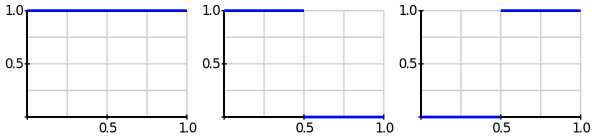
\includegraphics{5_b_Haar_1}} 
%\resizebox{!}{1.5in}{\includegraphics{phi_0_0}}  \hspace{0.1in} \resizebox{!}{1.5in}{\includegraphics{phi_1_0}} \hspace{0.1in} \resizebox{!}{1.5in}{\includegraphics{phi_1_1}} 
\end{center}
\caption{Graphs of $\phi(x)$, $\phi(2x)$, and $\phi(2x-1)$ from left to right.}
\label{F:phi_graphs_1}
\end{figure}

This function $\phi$ may seem to be a very simple function but it has properties that will be important to us. One property is that $\phi$ satisfies a scaling equation. For example, Figure \ref{F:phi_graphs_1} shows that 
\[\phi(x) = \phi(2x) + \phi(2x-1)\]
while Figure \ref{F:phi_graphs_2} shows that 
\[\phi(x) = \phi(2^2x) + \phi(2^2x-1) +  \phi(2^2x-2) + \phi(2^2x-3).\]
 \begin{figure}[h]
\begin{center}
\resizebox{!}{1.0in}{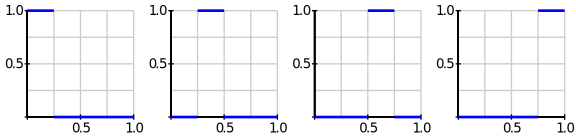
\includegraphics{5_b_Haar_2}}
%\resizebox{!}{1.15in}{\includegraphics{phi_2_0}} \hspace{0.05in} \resizebox{!}{1.15in}{\includegraphics{phi_2_1}} \hspace{0.05in} \resizebox{!}{1.15in}{\includegraphics{phi_2_2}}
% \hspace{0.05in} \resizebox{!}{1.15in}{\includegraphics{phi_2_3}}
\end{center}
\caption{Graphs of $\phi(2^2x)$, $\phi(2^2x-1)$, $\phi(2^2x-2)$, and $\phi(2^2x-3)$, from left to right.}
\label{F:phi_graphs_2}
\end{figure}
So $\phi$ is a sum of scalings and translations of itself.  In general, for each positive integer $n$ and integers $k$ between 0 and $2^n-1$ we define
\[\phi_{n,k}(x) = \phi\left(2^nx-k\right).\]
Then  $\phi(x) = \sum_{k=0}^{2^{n}-1} \phi_{n,k}(x)$ for each $n$.

These functions $\phi_{n,k}$ are useful in that they form a basis for the vector space $V_n$ of all piecewise constant functions on $[0,1]$ that have possible breaks at the points $\frac{1}{2^n}$, $\frac{2}{2^n}$, $\frac{3}{2^n}$, $\ldots$, $\frac{2^n-1}{2^n}$. This is exactly the kind of space in which digital signals live, especially if we sample signals at $2^n$ evenly spaced points on $[0,1]$. Let $\CB_n = \{ \phi_{n,k} : 0 \leq k \leq 2^n-1\}$. You may assume without proof that $\CB_n$ is a basis of $V_n$. 


\begin{pactivity} ~
	\ba
	\item Draw the linear combination $2\phi_{2,0} - 3\phi_{2,1} + 17 \phi_{2,2} + 30 \phi_{2,3}$. What does this linear combination look like? Explain the statement made previously ``Notice that these $2^n$ functions $\phi_{n,k}$ form a basis for the vector space of all piecewise constant functions on $[0,1]$ that have possible breaks at the points $\frac{1}{2^n}$, $\frac{2}{2^n}$, $\frac{3}{2^n}$, $\ldots$, $\frac{2^n-1}{2^n}$". 


	\item Remember that we can consider our data to represent a piecewise constant function obtained by partitioning $[0,1]$ into $n$ subintervals, where $n$ represents the number of sample points. Suppose we collect the following data: $10$, $13$, $21$, $55$, $3$, $12$, $4$, $18$. Explain how we can use this data to define a piecewise constant function $f$ on $[0,1]$. Express $f$ as a linear combination of suitable functions $\phi_{n,k}$. Plot this linear combination of $\phi_{n,k}$ to verify. 


	\ea
\end{pactivity}

Working with functions can be more cumbersome than working with vectors in $\R^n$, but the digital nature of our data makes it possible to view our piecewise constant functions as vectors in $\R^n$ for suitable $n$. More specifically, if $f$ is an element  in $V_n$, then $f$ is a piecewise constant function on $[0,1]$ with possible breaks at the points $\frac{1}{2^n}$, $\frac{2}{2^n}$, $\frac{3}{2^n}$, $\ldots$, $\frac{2^n-1}{2^n}$. If $f$ has the value of $y_i$ on the interval between $\frac{i-1}{2^n}$ and $\frac{i}{2^n}$, then we can identify $f$ with the vector $\left[y_1 \ y_1 \ \ldots \ y_{2^n}\right]^{\tr}$. 

\begin{pactivity} \label{act:wavelets_vectors} ~
\ba
\item Determine the vector in $\R^8$ that is identified with $\phi$. 


\item Determine the value of $m$ and the vectors in $\R^m$ that are identified with $\phi_{2,0}$, $\phi_{2,1}$, $\phi_{2,2}$, and $\phi_{2,3}$.


\ea

\end{pactivity}

We can use the functions $\phi_{n,k}$ to represent digital signals, but to manipulate the data in useful ways we need a different perspective. A different basis for $V_n$ (a \emph{wavelet basis}) will allow us to identify the pieces of the data that are most important. We illustrate in the next activity with the spaces $V_1$ and $V_2$. 

\begin{pactivity} \label{act:psi} The space $V_1$ consists of all functions that are piecewise constant on $[0,1]$ with a possible break at $x=\frac{1}{2}$. The functions $\phi = \phi_{n,k}$ are used to records the values of a signal, and by summing these values we can calculate their average. Wavelets act by averaging and differencing, and so $\phi$ does the averaging. We need functions that will perform the differencing.  
\ba
\item Define $\{\psi_{0,0}\}$ as 
	\[\psi_{0,0}(x) = \begin{cases}
	1 &\text{ if } 0 \leq x < \frac{1}{2} \\
	-1 &\text{ if } \frac{1}{2} \leq x < 1 \\
	0 &\text{ otherwise}
	\end{cases}.\]
	A picture of $\psi_{0,0}$ is shown in Figure \ref{F:psi_graphs}. Since $\psi_{0,0}$ assumes values of $1$ and $-1$, we can use $\psi_{0,0}$ to perform differencing. The function $\psi = \psi_{0,0}$ is the Mother Haar wavelet.\footnote{The first mention of wavelets appeared in an appendix to the thesis of A. Haar in 1909.} Show that $\{\phi, \psi\}$ is a basis for $V_1$. 
\begin{figure}[h]
\begin{center}
\resizebox{!}{1.0in}{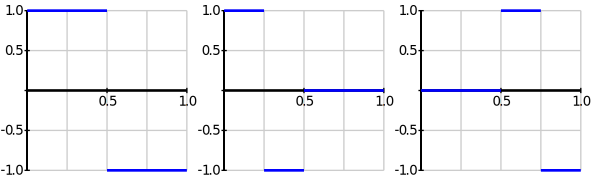
\includegraphics{5_b_Haar_3}}
%\resizebox{!}{1.5in}{\includegraphics{Haar_mother}} \hspace{0.1in} \resizebox{!}{1.5in}{\includegraphics{psi_1_0}} \hspace{0.1in} \resizebox{!}{1.5in}{\includegraphics{psi_1_1}}
\caption{The graphs of $\psi_{0,0}$, $\psi_{1,0}$ and $\psi_{1,1}$ from left to right.}
\label{F:psi_graphs}
\end{center}

\end{figure}
    

	\item We continue in a manner similar to the one in which we constructed bases for $V_n$. For $k=0$ and $k=1$, let $\psi_{1,k} = \psi\left(2^1x-k\right)$. Graphs of $\psi_{1,0}$ and $\psi_{1,1}$ are shown in Figure \ref{F:psi_graphs}. The functions $\psi_{1,k}$ assume the values of $1$ and $-1$ on smaller intervals, and so can be used to perform differencing on smaller scale than $\psi_{0,0}$. Show that $\{\phi_{0,0}, \psi_{0,0}, \psi_{1,0}, \psi_{1,1}\}$ is a basis for $V_2$. 


	\ea
\end{pactivity}

As Project Activity \ref{act:psi} suggests, we can make a basis for $V_n$ from $\phi_{0,0}$ and functions of the form $\psi_{n,k}$ defined by $\psi_{n,k}(x) = \psi\left(2^nx-k\right)$ for $k$ from 0 to $2^n-1$.  More specifically, if we let $\CS_n = \{\psi_{n,k} : 0 \leq k \leq 2^n-1\}$, then the set 
\[\CW_n = \{\phi_{0,0}\} \cup \bigcup_{j=0}^{n-1} \CS_j\]
is a basis for $V_n^{\perp}$ (we state this without proof). The functions $\psi_{n,k}$ are the \emph{wavelets}. 

\begin{pactivity} \label{act:wavelets_differencing} We can now write any function in $V_n$ using the basis $\CW_n$. As an example, the string 50, 16, 14, 28 represents a piecewise constant function which can be written as $50 \phi_{2,0} + 16 \phi_{2,1} + 14 \phi_{2,2} + 28 \phi_{2,3}$, an element in $V_2$. 
	\ba
	\item Specifically identify the functions in $\CW_0$, $\CW_1$, and $\CW_2$, and $\CW_3$. 


	\item As mentioned earlier, we can identify a signal, and each wavelet function, with a vector in $\R^m$ for an appropriate value of $m$. We can then use this identification to decompose any signal as a linear combination of wavelets. We illustrate this idea with the signal $[50 \ 16 \ 14 \ 28]^{\tr}$ in $\R^4$. Recall that we can represent this signal as the function $f = 50 \phi_{2,0} + 16 \phi_{2,1} + 14 \phi_{2,2} + 28 \phi_{2,3}$.
	\begin{enumerate}[i.]
	\item Find the the vectors $\vw_1$, $\vw_2$, $\vw_3$, and $\vw_4$ in $\R^m$ that are identified with $\phi_{0,0}$, $\psi_{0,0}$, $\psi_{1,0}$, and $\psi_{1,1}$, respectively.
	

	\item Any linear combination $c_1\phi_{0,0} + c_2 \psi_{0,0} + c_3 \psi_{1,0} + c_4\psi_{1,1}$ is then identified with the linear combination $c_1 \vw_1 + c_2 \vw_2 + c_3 \vw_3 + c_4 \vw_4$. Use this idea to find the weights to write the function $f$ as a linear combination of $\phi_{0,0}$, $\psi_{0,0}$, $\psi_{1,0}$, and $\psi_{1,1}$.
	

	
	\end{enumerate}

\ea

\end{pactivity}

Although is it not necessarily easy to observe, the weights in the decomposition $f = 27 \phi_{0,0} + 6 \psi_{0,0} + 17 \psi_{1,0} - 7 \psi_{1,1}$ are just averages and differences of the original weights in $f = 50 \phi_{2,0} + 16 \phi_{2,1} + 14 \phi_{2,2} + 28 \phi_{2,3}$. To see how, notice that if we take the overall average of the original weights we obtain the value of $27$. If we average the original weights in pairs ($50$ and $16$, and $14$ and $28$) we obtain the values $33$ and $21$, and if we take average differences of the original weights in pairs ($50$ and $16$, and $14$ and $28$) we obtain the values $17$ and $-7$. We can treat the signal $[33 \ 21]^{\tr}$ formed from the average of the pairs of the original weights as a smaller copy of the original signal. The average difference of the entries of this new signal is $6$. So the weights in our final decomposition are obtained by differences between successive averages and certain coefficients. The coefficients in our final decomposition $27 \phi_{0,0} + 6 \psi_{0,0} + 17 \psi_{1,0} - 7 \psi_{1,1}$ are called \emph{wavelet coefficients}. This is the idea that makes wavelets so useful for image compression. In many images, pixels that are near to each other often have similar coloring or shading. These pixels are coded with numbers that are close in value. In the differencing process, these numbers are replaced with numbers that are close to 0. If there is little difference in the shading of the adjacent pixels, the image will be changed only a little if the shadings are made the same. This results in replacing these small wavelet coefficients with zeros. If the processed vectors contain long strings of zeros, the vectors can be significantly compressed.  

Once we have recognized the pattern in expressing our original function as an overall average and wavelet coefficients we can perform these operations more quickly with matrices.


\begin{pactivity} \label{act:wavelets_matrices} The process of averaging and differencing discussed in and following Project Activity \ref{act:wavelets_differencing} can be viewed as a matrix-vector problem. As we saw in Project Activity \ref{act:wavelets_differencing}, we can translate the problem of finding wavelet coefficients to the matrix world. 
	\ba
	\item Consider again the problem of finding the wavelet coefficients contained in the vector $[27 \ 6 \ 17 \ - 7]^{\tr}$ for the signal $[50 \ 16 \ 14 \ 28]^{\tr}$. Find the matrix $A_4$ that has the property that $A_4 [50 \ 16 \ 14 \ 28]^{\tr} = [27 \ 6 \ 17 \ - 7]^{\tr}$. (You have already done part of this problem in Project Activity \ref{act:wavelets_differencing}.) Explain how $A_4$ performs the averaging and differencing discussed earlier.


	\item Repeat the process in part (a) to find the matrix $A_8$ that converts a signal to its wavelet coefficients. 



\item The matrix $A_i$ is called a \emph{forward wavelet transformation matrix} and $A_i^{-1}$ is the \emph{inverse wavelet transform matrix}. Use $A_8$ to show that the wavelet coefficients for the data string $[80 \ 48 \ 4 \ 36 \ 28 \ 64 \ 6 \ 50]^{\tr}$ are contained in the vector $[39.5 \ 2.5 \ 22 \ 9 \ 16 \ -16 \ -18 \ -22]^{\tr}$. 

	\ea
	
\end{pactivity}

Now we have all of the necessary background to discuss image compression. Suppose we want to store an image. We partition the image vertically and horizontally and record the color or shade at each grid entry. The grid entries will be our pixels. This gives a matrix, $M$, of colors, indexed by pixels or horizontal and vertical position. To simplify our examples we will work in gray-scale, where our grid entries are integers between 0 (black) and 255 (white). We can treat each column of our grid as a piecewise constant function. As an example, the image matrix $M$ that produced the picture at left in Figure \ref{F:Flower_1} is given in (\ref{eq:flower_image_matrix}). 

We can then apply a 16 by 16 forward wavelet transformation matrix $A_{16}$ to $M$ to convert the columns to averages and wavelet coefficients that will appear in the matrix $A_{16}M$. These wavelet coefficients allow us to compress the image -- that is, create a smaller set of data that contains the essence of the original image. 


Recall that the forward wavelet transformation matrix computes weighted differences of consecutive entries in the columns of the image matrix $M$. If two entries in $M$ are close in values, the weighted difference in $A_{16}M$ will be close to 0. For our example, the matrix $A_{16}M$ is  approximately
\[\left[\arraycolsep=1.0pt {\tiny{ \begin {array}{cccccccccccccccc}  208.0& 202.0& 178.0& 165.0&
 155.0& 172.0& 118.0& 172.0& 155.0& 153.0& 176.0& 202.0& 208.0& 210.0&
 209.0& 208.0\\ 33.4& 24.1&- 0.625& 0.938&- 2.50&-
 5.94& 42.8&- 5.94&- 2.50& 12.8& 0.938& 24.7& 30.6& 33.4& 32.5& 31.6
\\- 1.88&- 13.8& 19.4& 2.50& 0.0&- 2.50& 8.12&- 2.50
& 0.0& 2.50& 19.4&- 13.8& 1.88&- 3.75&- 1.88& 0.0\\
 17.5& 61.9& 61.9& 6.88& 0.0& 61.9& 0.0& 61.9& 0.0& 30.6& 65.0& 66.9&
 66.9& 19.4& 66.9& 66.9\\ 0.0& 27.5& 43.8& 16.2& 0.0
&- 11.2& 16.2&- 11.2& 0.0& 16.2& 43.8& 27.5& 0.0& 0.0& 0.0& 0.0
\\ 3.75& 0.0& 27.5&- 11.2& 0.0&- 16.2& 22.5&- 16.2&
 0.0&- 11.2& 27.5& 0.0&- 3.75&- 7.50&- 3.75& 0.0\\
 47.5& 0.0& 0.0& 13.8& 82.5& 0.0& 0.0& 0.0& 82.5& 13.8& 0.0& 3.75&
 3.75& 51.2& 3.75& 3.75\\ 82.5& 41.2& 41.2& 82.5&
 82.5& 41.2& 0.0& 41.2& 82.5& 35.0& 35.0& 35.0& 35.0& 82.5& 35.0& 35.0
\\ 0.0& 0.0& 0.0& 55.0&- 22.5&- 22.5& 55.0&- 22.5&-
 22.5& 55.0& 0.0& 0.0& 0.0& 0.0& 0.0& 0.0\\ 0.0&
 55.0&- 22.5&- 22.5& 22.5& 0.0&- 22.5& 0.0& 22.5&- 22.5&- 22.5& 55.0&
 0.0& 0.0& 0.0& 0.0\\- 7.50& 0.0&- 55.0& 22.5& 22.5&
- 22.5& 0.0&- 22.5& 22.5& 22.5&- 55.0& 0.0& 7.50& 0.0& 0.0& 0.0
\\ 0.0& 0.0& 0.0& 0.0& 22.5&- 55.0& 0.0&- 55.0& 22.5
& 0.0& 0.0& 0.0&- 15.0& 0.0&- 7.50& 0.0\\ 0.0& 0.0&
 0.0&- 55.0& 0.0& 0.0& 0.0& 0.0& 0.0&- 55.0& 0.0& 7.50& 7.50& 7.50&
 7.50& 7.50\\ 95.0& 0.0& 0.0&- 82.5& 0.0& 0.0& 0.0&
 0.0& 0.0&- 82.5& 0.0& 0.0& 0.0& 95.0& 0.0& 0.0\\
 0.0&- 82.5& 82.5& 0.0& 0.0&- 82.5& 0.0&- 82.5& 0.0& 95.0&- 95.0& 95.0
&- 95.0& 0.0& 95.0&- 95.0\\ 0.0& 0.0& 0.0& 0.0& 0.0&
 0.0& 0.0& 0.0& 0.0& 0.0& 0.0& 0.0& 0.0& 0.0& 0.0& 0.0\end {array} }}
 \right] .\]

Note that there are many wavelet coefficients that are quite small compared to others -- the ones where the weighted averages are close to 0. In a sense, the weighted differences tell us how much ``detail" about the whole that each piece of information contains. If a piece of information contains only a small amount of information about the whole, then we shouldn't sacrifice much of the picture if we ignore the small ``detail" coefficients. One way to ignore the small ``detail" coefficients is to use \emph{thresholding}.  

With thresholding (this is \emph{hard thresholding} or \emph{keep or kill}), we decide on how much of the detail we want to remove (this is called the \emph{tolerance}). So we set a tolerance and then replace each entry in our matrix $A_{16}M$ whose absolute value is below the tolerance with 0 to obtain a new matrix $M_1$. In our example, if you use a threshold value of 10 we obtain the new matrix $M_1$:
\[\left[\arraycolsep=1.0pt {\tiny{\begin {array}{cccccccccccccccc}  208.0& 202.0& 178.0& 165.0&
 155.0& 172.0& 118.0& 172.0& 155.0& 153.0& 176.0& 202.0& 208.0& 210.0&
 209.0& 208.0\\ 33.4& 24.1& 0.0& 0.0& 0.0& 0.0& 42.8
& 0.0& 0.0& 12.8& 0.0& 24.7& 30.6& 33.4& 32.5& 31.6
\\ 0.0&- 13.8& 19.4& 0.0& 0.0& 0.0& 0.0& 0.0& 0.0&
 0.0& 19.4&- 13.8& 0.0& 0.0& 0.0& 0.0\\ 17.5& 61.9&
 61.9& 0.0& 0.0& 61.9& 0.0& 61.9& 0.0& 30.6& 65.0& 66.9& 66.9& 19.4&
 66.9& 66.9\\ 0.0& 27.5& 43.8& 16.2& 0.0&- 11.2&
 16.2&- 11.2& 0.0& 16.2& 43.8& 27.5& 0.0& 0.0& 0.0& 0.0
\\ 0.0& 0.0& 27.5&- 11.2& 0.0&- 16.2& 22.5&- 16.2&
 0.0&- 11.2& 27.5& 0.0& 0.0& 0.0& 0.0& 0.0\\ 47.5&
 0.0& 0.0& 13.8& 82.5& 0.0& 0.0& 0.0& 82.5& 13.8& 0.0& 0.0& 0.0& 51.2&
 0.0& 0.0\\ 82.5& 41.2& 41.2& 82.5& 82.5& 41.2& 0.0&
 41.2& 82.5& 35.0& 35.0& 35.0& 35.0& 82.5& 35.0& 35.0
\\ 0.0& 0.0& 0.0& 55.0&- 22.5&- 22.5& 55.0&- 22.5&-
 22.5& 55.0& 0.0& 0.0& 0.0& 0.0& 0.0& 0.0\\ 0.0&
 55.0&- 22.5&- 22.5& 22.5& 0.0&- 22.5& 0.0& 22.5&- 22.5&- 22.5& 55.0&
 0.0& 0.0& 0.0& 0.0\\ 0.0& 0.0&- 55.0& 22.5& 22.5&-
 22.5& 0.0&- 22.5& 22.5& 22.5&- 55.0& 0.0& 0.0& 0.0& 0.0& 0.0
\\ 0.0& 0.0& 0.0& 0.0& 22.5&- 55.0& 0.0&- 55.0& 22.5
& 0.0& 0.0& 0.0&- 15.0& 0.0& 0.0& 0.0\\ 0.0& 0.0&
 0.0&- 55.0& 0.0& 0.0& 0.0& 0.0& 0.0&- 55.0& 0.0& 0.0& 0.0& 0.0& 0.0&
 0.0\\ 95.0& 0.0& 0.0&- 82.5& 0.0& 0.0& 0.0& 0.0&
 0.0&- 82.5& 0.0& 0.0& 0.0& 95.0& 0.0& 0.0\\ 0.0&-
 82.5& 82.5& 0.0& 0.0&- 82.5& 0.0&- 82.5& 0.0& 95.0&- 95.0& 95.0&-
 95.0& 0.0& 95.0&- 95.0\\ 0.0& 0.0& 0.0& 0.0& 0.0&
 0.0& 0.0& 0.0& 0.0& 0.0& 0.0& 0.0& 0.0& 0.0& 0.0& 0.0\end {array} }}
 \right]. \]

We now have introduced many zeros in our matrix. This is where we compress the image. To store the original image, we need to store every pixel. Once we introduce strings of zeros we can identify a new code (say 256) that indicates we have a string of zeros. We can then follow that code with the number of zeros in the string. So if we had a string of 15 zeros in a signal, we could store that information in 2 bytes rather than 15 and obtain significant savings in storage. This process removes some detail from our picture, but only the small detail. To convert back to an image, we just undo the forward processing by multiplying our thresholded matrix $M_1$ by $A_{16}^{-1}$. The ultimate goal is to obtain significant compression but still have $A_{16}^{-1}M_1$ retain all of the essence of the original image. 

In our example using $M_1$, the reconstructed image matrix is $A_{16}^{-1}M_1$ (rounded to the nearest whole number) is 
\[ \left[\arraycolsep=2.5pt  \begin {array}{cccccccccccccccc}  242& 240& 241& 237&
 132& 138& 232& 138& 132& 238& 239& 240& 238& 244&
 242& 240\\ 242& 240& 241& 127& 178&
 183& 122& 183& 178& 128& 239& 240& 238& 244& 242&
 240\\ 242& 240& 131& 127& 178& 183&
 122& 183& 178& 128& 129& 240& 238& 244& 242& 240
\\ 242& 130& 176& 172& 132& 183& 167&
 183& 132& 172& 174& 130& 238& 244& 242& 240
\\ 242& 240& 131& 177& 178& 133& 183&
 133& 178& 178& 129& 240& 238& 244& 242& 240
\\ 242& 240& 241& 132& 132& 178& 183&
 178& 132& 132& 239& 240& 238& 244& 242& 240
\\ 242& 240& 131& 177& 178& 133& 138&
 133& 178& 178& 129& 240& 223& 244& 242& 240
\\ 242& 240& 131& 177& 132& 243& 138&
 243& 132& 178& 129& 240& 253& 244& 242& 240
\\ 240& 240& 239& 124& 238& 234& 75&
 234& 238& 130& 241& 244& 244& 248& 244& 244
\\ 240& 240& 239& 234& 238& 234& 75&
 234& 238& 240& 241& 244& 244& 248& 244& 244
\\ 240& 240& 239& 69& 73& 234& 75&
 234& 73& 75& 241& 244& 244& 240& 244& 244
\\ 50& 240& 239& 234& 73& 234& 75&
 234& 73& 240& 241& 244& 244& 50& 244& 244
\\ 240& 75& 239& 248& 238& 69& 75&
 69& 238& 240& 51& 240& 50& 240& 240& 50
\\ 240& 240& 74& 248& 238& 234& 75&
 234& 238& 50& 241& 50& 240& 240& 50& 240
\\ 75& 75& 74& 83& 73& 69& 75& 69&
 73& 75& 76& 75& 75& 75& 75& 75\\
 75& 75& 74& 83& 73& 69& 75& 69& 73& 75& 76&
 75& 75& 75& 75& 75\end {array}  \right].\]


We convert this into a gray-scale image and obtain the image at right in Figure \ref{F:Flower_1}. Compare this image to the original at right in Figure \ref{F:Flower_1}. It is difficult to tell the difference.

There is a Sage file you can use at 
\begin{center} \url{http://faculty.gvsu.edu/schlicks/Wavelets_Sage.html}  \end{center}
that allows you to create your own 16 by 16 image and process, process your image with the Haar wavelets in $\R^{16}$, apply thresholding, and reconstruct the compressed image. matrix. You can create your own image, experiment with several different threshold levels, and choose the one that you feel gives the best combination of strings of 0s while reproducing a reasonable copy of the original image. 

		


